\documentclass{ATLAS_latex/atlasnote} 
\skipbeforetitle{-5pt}

\usepackage{graphicx,multirow}
\usepackage{epstopdf}
\usepackage{authblk}
\usepackage{hyperref}
\usepackage{pdfpages,subfigure,caption,placeins}
\usepackage{color}

\newcommand{\red}[1]{\textcolor[rgb]{1,0,0}{#1}}

%\newcommand{\et}{\mbox{$E_{T}$}}
%\newcommand{\met}{\mbox{$\protect \raisebox{.3ex}{$\not$}\et$}}
%\newcommand{\ppbar}{\mbox{$p\overline{p} \ $}}
\newcommand{\pbarp}{\mbox{$\overline{p}p$}}
\newcommand{\hs}{\hspace*{0.375in}}
\newcommand{\zmumu}{\mbox{$Z \rightarrow \mu\mu$}}
\newcommand{\zee}{\mbox{$Z \rightarrow ee$}}
\newcommand{\psimumu}{\mbox{J/$\psi \rightarrow \mu\mu$}}
\newcommand{\oopsmumu}{\mbox{$\Upsilon \rightarrow \mu\mu$}}
%\newcommand{\mtop}{\mbox{$M_{top}$}}
\newcommand{\pt}{\mbox{P_{T}}}
\newcommand{\topq}{\mbox{${\rm top-quark}$}}
\newcommand{\topdecaylj}{$ \overline{t}$}
%\newcommand{\tt}{$ t \bar t$}
%\newcommand{\ttbar}{$t\bar{t} \ $}
\hyphenation{posi-trons in-di-rect-ly mod-el-ling}

%
% Input some definitions
%
%
%----------  PHYSICS COMMANDS
%
\def \Et {{\rm E}_{\rm T}}
\def \Pt {{\rm P}_{\rm T}}
\def \Pz {{\rm P}_{\rm Z}}
\def \enu {\epsilon_{\nu}}
\def \stw {$\sin^{2}\theta_{W}$}
\newcommand{\MET}{\mbox{$\protect \raisebox{.3ex}{$\not$}\et$}}
\newcommand{\METC}{\mbox{$\protect \raisebox{.3ex}{$\not$}\etc$}}
%\def \MET {\not\!\Et}
\def\deg{^\circ}
\def\qbar{{\bar q}}
\def\nubar{{\bar \nu}}
\def\W{{\em W\/ }}
\def\Z0{${\em Z^0\/}$}
\def \lum {{\cal L}}
\def\epem{{\rm e^{+}e^{-}}}
\def\tptm{{\tau^{+}\tau^{-}}}
\def\roots{${\sqrt s}\:$}
\def\r#1 {$^{#1}$}
\def\sigW {$\sigma\cdot$B(\W$\rightarrow~$e $\nu$) }
\def\sigZ {$\sigma\cdot$B(\Z0$\rightarrow~\epem$) }
\hyphenation{brem-sstrah-lung proc-ess}
%
\def\first{{\mbox{$I\leq$}4~GeV}}
\def\second{{QC=\mbox{$I\leq$}~4~GeV+\mbox{$s_{ip}\leq$}~4}}
\def\third{{QC+\mbox{$\delta \phi \geq 2$}}}
\def\fourth{{QC+\mbox{$|\cos \theta^{*}| \leq 0.4$}}}
\def\fifth{{QC+\mbox{$\delta \phi \geq 2$}+\mbox{$|\cos \theta^{*}|\leq 0.4$}}} 
\def\six{{QC+\mbox{$\sum p_t  \leq$}40~GeV+\mbox{$\sum s_{ip} \leq 30$}}}
\def\seven{{\mbox{$\delta \phi \geq 2$}}}
\def\eight{{\mbox{$|\cos \theta^{*}| \leq 0.4$}}}
\def\nine{{\mbox{$\delta \phi \geq 2$}+\mbox{$|\cos \theta^{*}| \leq 0.4$}}} 
%
%\input moredefs.tex
%
%
%
%
\newcommand{\etc}{{\rm E}_{\scriptscriptstyle\rm T}^{\scriptscriptstyle\rm C}}
\newcommand{\et}{{\rm E}_{\scriptscriptstyle\rm T}}
\newcommand{\etcone}{{\rm E}_{\scriptscriptstyle\rm T}^{cone}}
\newcommand{\abseta}{\mid \eta^{det} \mid \leq}
\newcommand{\abz}{\mid z \mid \leq}
\newcommand{\fb}{f_{b}}
\newcommand{\ks}{K_{s}^{0}}
\newcommand{\pich}{\pi^{\pm}}
\newcommand{\piz}{ \pi^{0} }
\newcommand{\bigz}{{\cal Z}}
\newcommand{\emf}{f_{em}}
\newcommand{\deltar}{\sqrt{\Delta \eta ^{2}+ \Delta \phi ^{2}}}
\newcommand{\etprime}{{\rm E}_{\scriptscriptstyle\rm T'}}
\newcommand{\ptran}{{\rm P}_{\scriptscriptstyle\rm T}}
\newcommand{\met}{\mbox{$\protect \raisebox{.3ex}{$\not$}\et \ $}}
\newcommand{\wenu}{W \rightarrow e \nu}
\newcommand{\wmunu}{W \rightarrow \mu \nu}
\newcommand{\wlep}{W \rightarrow \rm{lepton}\, \nu}
\newcommand{\zv}{{\rm z}_{vertex}}
\newcommand{\wbb} {W b\bar{b} }
\newcommand{\wcc} {W c\bar{c} }
\newcommand{\ppbar}{p\bar{p}}
\newcommand{\qqbar}{q\bar{q}}
\newcommand{\ttbar}{t\bar{t}}
\newcommand{\bbbar}{b\bar{b}}
\newcommand{\ccbar}{c\bar{c}}
\newcommand{\ppbb} { \ppbar \rightarrow  \bbbar }
%\newcommand{\zee}{Z \rightarrow e^{+}e^{-} }
\newcommand{\bele}{b \rightarrow c e \nu_{e} }         
\newcommand{\blnu}{b \rightarrow c l \nu_{l} }         
\newcommand{\mtran}{{\rm M}_{\scriptscriptstyle\rm T}}
\newcommand{\acceff}{\rm{A} \times \epsilon}
\newcommand{\bbar} {\bar{b}}   
\newcommand{\gbb} { g \rightarrow b\bar{b} }
\newcommand{\gcc} { g \rightarrow c\bar{c}}
\newcommand{\tbar} { \bar{{t}}  }                                
\newcommand{\Lik}{\mbox{$\mathcal{L}$ }}
\newcommand{\Ki}{\mbox{$\chi^{2}$ }}
\newcommand{\mPr}{\mathcal{P}}
\newcommand{\CPr}{\mbox{$\mathcal{C}$ }}
\newcommand{\mLik}{\mathcal{L}}
\newcommand{\mCPr}{\mathcal{C}}
% dilepton symbols1
\def \mc {\multicolumn}
\def \pb    {pb$^{-1} $}
\def \DeltaPhi {$\Delta \phi_{\ell\,\ell \ }$} 
\def \mtop {$M_{top} \ $}
\def \mtopev {$M_{top}^{event} $}
\def \mw {$M_{W} \ $}
\def \ztau   {$Z\rightarrow\tau\tau \:$}
\def \DeltaPhil {$\Delta \phi{(\MET,\ell) \ }$} 
\def \DeltaPhij {$\Delta \phi{(\MET,j) \ }$} 
\def \TTbar {$t\overline{t} \; \;$}
\def \dpemu {\Delta \phi_{e\mu}}
\def \Mt {M_{top}}
\def \mtenu  {M_{T}^{e\nu}}
\def \lum {\cal L}
\def \intlum {\int {\cal L} dt}
\def \Zee {Z^{0} \rightarrow e^{+}e^{-}}
\def \Zmumu {Z^{0} \rightarrow \mu^{+}\mu^{-}}
\def \emu {e \mu}  
\def \temux {\ttbar \rightarrow \emu + X}
\def \tljx {\ttbar \rightarrow \ell \nu q \bar{q}^{\prime} b \bar{b} X}
\def \tllx {\ttbar \rightarrow \ell^+ \bar{\nu} \ell^- \nu b \bar{b} X}
\def \thad {\ttbar \rightarrow q \bar{q} b q \bar{q} \bar{b} X}   
\def \Ete {E_T^{e}}
\def \Ptmin {P_T^{min}}
\def \Ptmu {P_T^{\mu}}
\def \Etmiss {{\not}{E_T}}
% end of dilepton
%---------- UNITS, SYMBOLS
%
\newcommand{\imb}{ \mu {\rm b}^{-1} }
\newcommand{\inb}{ {\rm nb}^{-1} }
\newcommand{\ipb}{ {\rm pb}^{-1} }
\newcommand{\degs}{\mbox{$^{\circ}$}}
\newcommand{\gsim}{\mbox{\small$\stackrel{>}{\sim}$\normalsize}}
\newcommand{\lsim}{\mbox{\small$\stackrel{<}{\sim}$\normalsize}}
\newcommand{\gev}  { {\rm GeV}}
\newcommand{\tev}  { {\rm TeV}}
\newcommand{\gevc} { {\rm GeV/c}}
\newcommand{\gevcc}{ {\rm GeV/c^2}}

%
%---------- TYPE SETTING
%
\newcommand{\etal}{{\em et al.}}
\newcommand{\tableskip}{\vskip 5pt plus3pt minus1pt \relax}
\newcommand{\tindent}{\hskip 17pt}
\newcommand{\hfull}{\hspace*{\fill}}
\newcommand{\tline}{\protect\linebreak[4]\hfull}
\newcommand{\linespace}[1]{\protect\renewcommand{\baselinestretch}{#1}
  \footnotesize\normalsize}
%
%---------- Journal names
%
%\newcommand{\prl}[1]{Phys. Rev. Lett {\bf #1}}
%\newcommand{\prev}[1]{Phys. Rev. {\bf #1}}
%\newcommand{\prd}[1]{Phys. Rev. D {\bf #1}}
%\newcommand{\zs}[1]{Z. Phys. {\bf #1}}
%\newcommand{\ncim}[1]{Nuovo Cim. {\bf #1}}
%\newcommand{\plet}[1]{Phys. Lett. {\bf #1}}
%\newcommand{\prep}[1]{Phys. Rep. {\bf #1}}
%\newcommand{\rmp}[1]{Rev. Mod. Phys. {\bf #1}}
%\newcommand{\nphy}[1]{Nucl. Phys. {\bf #1}}
%\newcommand{\nim}[1]{Nucl. Instrumen. Meth. {\bf #1}}
%

%------------- Figure commands and macros
%
%
%  Called the same way epsffile is called.  Difference is it will center
%  the graphic in the page useing the center environment.
%
\def\gepsfcentered#1{
  \def\testit{#1}
  \def\lbracket{[}
  \ifx\testit\lbracket
    \let\dofilecmd=\gepsfwithopt
  \else
    \let\dofilecmd=\gepsfnoopt
  \fi
  \dofilecmd}

\def\gepsfnoopt#1{
  \begin{center}
  \leavevmode
  \epsffile{#1}
  \end{center}}

\def\gepsfwithopt#1 #2 #3 #4]#5{
  \begin{center}
  \leavevmode
  \gepsfmaxx=0.94\textwidth
  \epsffile[#1 #2 #3 #4]{#5}
  \end{center}}

%
%  Auto sizing for epsf figures that are larger than the text width.
%
\newdimen\gepsfmaxx
\gepsfmaxx=0.94\textwidth
\def\epsfsize#1#2{
  \ifnum \epsfxsize=0
    \ifnum \epsfysize=0
      \ifnum #1 > \gepsfmaxx
        \gepsfmaxx
	%\message{Did scaling.}
      \else
        #1
	%\messaeg{Used nat scaling}
      \fi
    \else
      \epsfxsize
      %\message{Using what ever.}
    \fi
  \else
    \epsfxsize
    %\message{Again, using whatever.}
  \fi
  %\message{Hi epsfxsize is \the\epsfxsize ...}
  %\message{epsfysize is \the\epsfysize ...}
  %\message{Hi first arg is \the#1 ...}
  %\message{Second arg is \the#2 ...}
}


\renewcommand{\topfraction}{0.95}
\renewcommand{\bottomfraction}{0.8}
\renewcommand{\textfraction}{0.06}
\renewcommand{\floatpagefraction}{0.85}
\setcounter{totalnumber}{5}
\setcounter{topnumber}{4}

\bibliographystyle{apsrev}

\title {Test of the Micromegas Trigger Processor with Cosmic Ray Muons}

\usepackage{authblk}
\renewcommand\Authands{, } % avoid ``. and'' for last author
\renewcommand\Affilfont{\itshape\small} % affiliation formatting
\author[a]{J.~Farah}
\author[a]{N.~Felt}
\author[a]{M.~Franklin}
\author[a]{P.~Giromini}
\author[a]{J.~Philion}
\author[a]{A.~Tuna}
\author[a]{A.~Wang}
\affil[a]{Harvard University, Cambridge, Massachusetts 02138, USA}

\abstracttext{\noindent We have commissioned a MM Trigger Processor demonstrator
 after adding ART Data-Driver Cards 
 to the existing Harvard Micromegas octuplet instrumented with MMFE8 front-end boards.
 The MMTP spatial and time resolutions are measured using cosmic muons with energy $\ge 0.8$~GeV$/c^2$.}

\clearpage


\begin{document} 

\setcounter{page}{2}

\section{Introduction}
\label{sec:intro}

We investigate the performance of the micromegas Address in Real Time (ART) and trigger processor. This is one of the two trigger technologies introduced for the New Small Wheel (NSW) upgrade of the ATLAS muon spectrometer, which is intended to be built and installed in the coming years. 

The performance is measured with hundreds of thousands of cosmic muons recorded at the Harvard cosmic ray test stand, which employs a full trigger electronics path with prototype hardware: MMFE8s equipped with VMM2, the FPGA-based ADDC V1, and a micromegas trigger processor (MMTP) implemented on a VC707 FPGA evaluation board.

This note presents the performance of the trigger data path; the full readout data path is described in previous notes~\cite{noisy,noiseless} using the same detectors and similar electronics. The reader is encouraged to read these notes for complementary measurements and a better understanding of the performance of the micromegas detectors and electronics in a broader context.


\section{Experiment}
\label{sec:exp}

The experiment is micromegas.

\subsection{Micromegas and scintillator detectors}
\label{sec:exp-mm}

\subsection{Electronics}
\label{sec:exp-elx}

\subsubsection{Hardware}
\label{sec:exp-hw}

The micromegas readout paths includes three separate cards. The MMFE8 is the front-end readout card, and it houses 8 VMM2 ASICs per card. These readout chips receive signals from the detector and digitize them, and they are discussed in great detail elsewhere~\cite{nswtdr,noisy,noiseless}. The MMFE8 also houses an FPGA for configuring and reading out the VMMs over ethernet. The experiment in this note has 8 layers of micromegas detectors and therefore 8 MMFE8s.

The ART Data Driver Card (ADDC) is a driver card for the micromegas trigger data path. It receives data from 4 MMFE8s over mini-SAS connections and packages this data into a single output for downstream clients. The card houses an FPGA for this purpose. There are 2 ADDCs in this experiment to receive data from the 8 MMFE8s.

The Micromegas Trigger Process (MMTP) is the last card of the micromegas trigger path. It receives data from ADDCs over fiber optical connections and interrogates the data for the presence of triggers. The card houses an FPGA for this purpose. There is 1 MMTP in this experiment to receive data from the 2 ADDCs.

Additionally, a board was built at Harvard for the purpose of operating the MMFE8s synchronously, referred to as the clock/trigger board. This board sends a 40 MHz clock to all 8 boards, which are used by each board as a mother clock, thereby synchronizing them. The board also receives trigger signals from the scintillator and distributes them to the MMFE8s, as discussed in Section~\ref{sec:exp-mmfe}.

\subsubsection{Trigger data path}
\label{sec:exp-art}

The micromegas trigger data path begins at the VMM. The data path is referred to as the Address in Real Time (ART) data path, which refers to the output of the VMM. The full readout can include many strips per BC, and each strip read out includes lots of information about the strip, including charge (PDO) and time (BCID, TDO). Alternatively, the trigger readout sends the data from at most one strip per BC, and it only includes the address of the strip. This is the crux of the trigger data path; the bandwidth of the trigger data path is greatly reduced relative to the full readout. One bit is used to announce a hit is recorded, and six bits are used for the address.

The VMM has two operating modes for the ART: at-threshold and at-peak. These modes describe the time at which an ART signal is sent by the VMM. Threshold mode is faster than peak mode because the VMM sends the signal as soon as a threshold is crossed, instead of waiting until a peak is found. The data in this note are taken with the ART operating at threshold.

The VMM sends ART data over mini-SAS cables to the ART Data-Driver Card (ADDC), which collects ART signals from 4 MMFE8 and packages them into a single output. The ART data bypasses the MMFE8 readout chip entirely. The data in this note are taken with ADDC V1, in which the ADDC has an on-board FPGA for collecting and packaging the incoming signals. The final version of the ADDC will have an on-board ASIC for this purpose, since it will be mounted in the ATLAS cavern and must be radiation tolerant. However, the functionality of the FGPA-based and ASIC-based ADDC are expected to be identical.

The ADDC then sends the packaged ART data to the micromegas trigger processor (MMTP). The communication protocol is ``GBT'', which is developed at CERN and used by many experiments, and sent over fiber optic cables. The MMTP collects ART signals, analyzes them for patterns resembling a trigger, and sends trigger information to downstream clients. These steps are performed by an FPGA. The data in this note are taken with an implementation of the MMTP on a Xilinx VC707 development board with a Virtex-7 FPGA.

In this setup, 2 ADDCs are placed near the detector and accept ART signals from the 8 MMFE8s. The VC707 is placed further from the detector in a counting room, along with the DAQ computer and scintillator readout electronics. It accepts signals from both ADDCs.

\subsubsection{MMFE8 and scintillator data path}
\label{sec:exp-mmfe}

The MMFE8 and scintillator data paths are described in detail elsewhere~\cite{noisy,noiseless}. In brief, the DAQ computer communicates directly with the MMFE8s over ethernet connection. The full MMFE8 readout includes charge and time information for each strip above threshold in the form of PDO, TDO, and BCID. The MMFE8 only sends data over ethernet after it has received a trigger signal from the scintillator. The signal is sent from the scintillator to the clock/trigger board over coaxial cable with BNC connections, and the clock/trigger board sends this signal to the 8 MMFE8s over microHDMI.

The scintillator trigger is formed with a coincidence of six signals corresponding to the top, middle, and bottom scintillator counters. The signals are acquired by Lecroy TDC and sent to a CAMAC crate controller, which then sends its data over ethernet to the DAQ computer.

\subsubsection{Scintillator timestamp}
\label{sec:exp-scitime}

Additionally, there is a connection between the scintillator electronics and the MMTP, to utilize the fast internal clocks of the MMTP FPGA. The scintillator trigger signal is sent directly to the MMTP, which captures the signal using a 640 MHz clock and forwards this timestamp to the DAQ computer over ethernet. This is referred to as the \textit{scintillator timestamp}. It provides a more accurate reference time than the scintillator BCID captured by the MMFE8s, since the 640 MHz clock of the MMTP allows for $\sim\!1.56$ ns resolution, versus the $\sim\!25$ ns resolution of the 40 MHz clock.


\section{MM TP Algorithm}
\label{sec:alg}

The MM TP algorithm is designed to receive ART data transmitted via optical fiber using the GBT protocol, decode the ART data, filter the ART data into subsets (``triggers'') of ART data which satisfy a spatial and temporal coincidence, and calculate quantities which describe these triggers. The first step is referred to as the \textit{decoder}, the second step is referred to as the \textit{finder}, and the third step is referred to as the \textit{fitter}.

The MM TP algorithm is written in firmware and placed on a Xilinx Virtex-7 FPGA, which is housed by a VC707 evaluation board. The algorithm meets timing requirements for synthesis and implementation of the algorithm on the FPGA. Ultimately, the algorithm will be placed on a larger FPGA on a high-density optical mezzanine card (``HORX'') which will be housed in an ATCA shelf. The VC707 implementation is already capable of testing many aspects of the algorithm, however, including the steps mentioned above.

\subsection{Decoding}
\label{sec:alg-decode}

ART data is transmitted from the ADDC to the MM TP using the GBT protocol via optical fibers. The data is transmitted as a 128-bit word per BC. 12 bits describe the BCID; 32 bits describe which of the 32 VMMs associated with one ADDC are transmitting an ART signal; 48 bits give a maximum of 8 ART strip numbers, which are 6 bits each; and the remaining bits are used for checking data quality, such as an 8-bit data parity word.

After receiving the ART data, the MM TP converts the VMM and strip numbers into global strip numbers, also taking into consideration that some of the MM chambers are flipped relative to each other. For example, if an ART strip from VMM 5 is reported as strip number 30, the MM TP converts this to a global strip number of 350 ($5*64 + 30$). The units of the MM TP are strip pitches, and there is no conversion to a unit of meters. The MM TP then adds the distance from the beamline to the base of the MM chamber, in units of strips, to the global strip number, and divides the global strip number by the $z$-position of the chamber, to convert the strip to a slope, $x_\text{strip} / z_\text{strip}$.

\subsection{Adjustments for cosmic muons}
\label{sec:alg-crts}

The use of \textit{slopes} instead of \textit{strips} is motivated by the knowledge that particles arriving at the NSW from a proton-proton collision should travel in a nearly straight line. Thus, each layer of MM will record a different strip address for the incident particle, but a nearly identical slope. This simplifies logic for defining spatial \textit{roads} in the MM chamber.

However, for a cosmic ray test stand, the exact origin of incident particles are unknown. The MM TP algorithm is then modified to use strip addresses instead of slopes for the defintion of roads, as discussed in Section~\ref{sec:alg-finder}. The implementation of strip-to-slope conversion in the FPGA is nonetheless tested by multiplying each strip address by 1, instead of $1/z_\text{strip}$, to calculate a ``slope'' which is suitable for spatial coincidences of cosmic muons.

Additional adjustments to the MM TP algorithm for use at the cosmic ray test stand include: 

\subsection{Finder}
\label{sec:alg-finder}

Once the ART data is received and decoded, the next step of the MM TP algorithm is to filter the data into subsets which roughly look like an incident particle traversing the octuplet. This step is called the \textit{finder}.

The finder relies on heavy parallelization. A configurable number of roads are created in the FPGA to span the octuplet, and each roads evaluates in parallel whether is contains a sufficient number of ART strips to form a trigger. In this note, the road size is 1 road per VMM. This is demonstrated graphically in Figure~\ref{}.

Additionally, the roads should overlap to avoid edges cases where the incident muon travels very near to the boundary of two roads. This is implemented in the finder by allowing each road to use hits not only in their respective road, but also in neighboring roads. The number of neighboring roads is a configurable parameter; in this note, hits from one neighbor above and one neighbor below are used in a given road. For example, road 3 uses hits from VMM 2, VMM 3, and VMM 4, so that the effective road size is 3 VMMs.

The effective road size is chosen to maximize the acceptance of cosmic ray muons in the octuplet. 

A road must contain at least two hits on horizontal ($X$) planes and at least two hits on stereo ($UV$) planes to be satisfy a trigger. Additionally, at least two of the hits on $X$-planes must occur on opposite quadruplets, to ensure a good lever arm when fitting the $X$-hits to a line. These requirements are looser than the expected coincidence requirements at the NSW ($3X$ AND $3UV$), since the rate of noise and background hits is much lower for cosmic data-taking than at the LHC.

The finder also requires hits for a trigger to be within a time window in units of the BC clock. The expected time window for the NSW is two BCs; in this note, the window is increased to seven BCs to maximize efficiency and measure the efficiency of the window as a function of the size of the window. The time window is implemented as follows. When a hit arrives at the finder, it is stored in memory for seven BCs. For each road satisfied by the hit, no new hits are allowed in that road for that board until the hit is ``old'', i.e., after seven BCs. The stipulation that a hit in a road on a board cannot be overwritten by a new hit is motivated by the behavior of the detector and the ART data-flow: an incident muon is expected to leave a signal on multiple strips on a board (making a ``cluster''), each strip of which can send an ART signal typically separated by a couple of BCs. Only the first hit from the cluster should be used for the trigger, hence the earlier hit should not be overwritten by subsequent nearby hits. Then, as hits arrive, the coincidence requirements are evaluated for all roads in parallel. Once the coincidence requirements for a road are met and the earliest hit in the road becomes ``old'', a trigger is formed. Therefore hits are collected in a time window of seven BCs, and triggers cannot be formed until the oldest hit in the road is sufficiently old.

Every road is capable of forming one trigger per cycle of the BC clock. After evaluating all roads in parallel, the triggers created are placed in a priority encoder to be sent sequentially to the fitter for further calculations. The priority encoder sorts the triggers by road number, with smallest roads treated first. Because the MM TP clock is eight times faster than the BC clock, there can be at most eight triggers per BC.

\subsection{Fitter}
\label{sec:alg-fitter}

The triggers found by the finder are then sent to the \textit{fitter}, which calculates quantities of interest for the trigger. The fitter does not create or remove any triggers. The NSW implementation of the fitter is described first, and modifications for cosmic data-taking are described second.

For the NSW, the main deliverables of the fitter are the location and quality of a trigger. The location is represented by a region of interest (ROI), which is a number provided by downstream clients like Sector Logic mapping to $\eta-\phi$ space. The quality of the trigger is represented by the difference in angle a \textit{local} fit of the trigger ART hits and a \textit{global} fit. A \textit{local} fit is performed on only the ART hits, and a \textit{global} fit is performed with the constraint that the trigger be consistent with the interaction point.

The location of the trigger is derived in a Cartesian $m_x-m_y$ space, where $\hat{y}$ points perpendicular to the direction of the $X$-strips, $\hat{x}$ points parallel to the $X$-strips, and $m_i$ is the slope $i/z$\footnote{We apologize for the confusing notation. To recap: $X$, $U$, and $V$ denote different layers of micromegas. $x$, $y$, and $z$ are cartesian coordinates. The $X$-layers measure $m_y$.}. $m_y$ is measured as the average of slopes measured in each $X$-plane, $\overline{m_X}$. $m_x$ is measured as the difference between slopes measured in the $U$ and $V$ planes, with a geometric factor from the angle of the stereo strips: $\frac{m_U - m_V}{2\ \text{tan}(\theta_\text{stereo})}$.

\subsection{Output}
\label{sec:alg-output}

Finally, the MM TP algorithm stores copies of the input ART data and output trigger data in FIFO buffers, which are transmitted as UDP packets via ethernet to a computer for analysis.

\subsection{Bugs encountered}
\label{sec:alg-bugs}

By January 2017, the MM TP algorithm had been implemented in firmware and successfully created triggers in behavioral simulation. By summer 2017, the MM TP algorithm is implemented on a FPGA and records hundreds of thousands of cosmic muon triggers per day. Many bugs were uncovered along the way.



\section{Data-taking}
\label{sec:data-taking}

The data described in this note was taken from May 2017 until July 2017. Each continuous period of data-taking is referred to as a ``run'', and the runs are described in Table~\ref{tab:runs}. 

The astute reader will notice there are many more MM TP events than MM FE events. There are three reasons for this. First, the MM TP sends data whenever the finder creates a trigger, whereas the MM FE only sends data when it receives a trigger signal from the scintillator. The MM TP then records many more triggers due to low energy cosmic muons, cosmic muons which miss the scintillators, and random noise which happens to satisfy the loosened trigger requirements. Run 3522 in particular observed more triggers from noise than the other runs. Second, the MM TP will typically make a handful of triggers for a single cosmic muon passing through the detector due to the overlapping roads. For example, a downward-going muon passing entirely through road 2 will make triggers in roads 1, 2, and 3. Third, if the incoming ART data is spread across many BCs, the MM TP will often make triggers on multiple BCs as the hits arrive. 

These last two circumstances are an open issue of the firmware logic, and duplicates will likely need to be removed from the MM TP before being sent to the sTGC trigger processor. In this note, if many triggers are created by the MM TP to describe a single muon, the trigger with the most hits is chosen for analysis.

Between Runs 3522 and 3527, two front-end cards were repaired and replaced on the detector. Therefore the data from Run 3522 is presented as the default performance in Section~\ref{sec:perf}, whereas the data from Runs 3527, 3528, and 3530 are used for comparing the performance for different integration times in Section~\ref{sec:perf-integ}

\begin{table}[!htpb]
\begin{center}
  \begin{tabular}{c | c | c | c | c}
    Run  & Dates         & MMFE Events & MMTP Events & Notes \\
    \hline
    3522 & 05/11 - 05/18 & 296532      & 15774567    & 200 ns integration time \\
    3527 & 06/26 - 07/02 & 233645      & 3635093     & 100 ns integration time \\
    3528 & 07/02 - 07/07 & 205053      & 3253330     & 50 ns integration time \\
    3530 & 07/19 - 07/24 & 192114      & 4060891     & 200 ns integration time \\
  \end{tabular}
  \caption{Information about each run of data-taking.}
\label{tab:runs}
\end{center}
\end{table}

% \subsection{Monitoring}
% \label{sec:data-mon}

\subsection{Readout errors}
\label{sec:data-errors}

\subsection{Combining data streams}
\label{sec:data-streams}

Three data streams are produced by the MM TP and written to disk, in addition to the scintillator and MMFE data streams. Two of the MM TP streams are written when a trigger is found. First, the trigger itself is output, which includes a BCID of the trigger, the ART hits of the trigger, and the quantities describing the trigger which are produced by the fitter. Second, all of the incoming ART hits in a window of 15 BCs around the trigger are output. The BCIDs of the hits used by the trigger are extracted from the second stream, and it is additionally useful for debugging the behavior of the algorithm offline. The third stream is independent of the algorithm, and it writes a 16-bit BCID to disk whenever it receives a trigger from the scintillator. This stream runs on a 640 MHz clock and allows for offline comparison of the TP trigger BCID to the scintillator BCID in steps of 1.56 ns.

All streams are synchronized and combined offline by comparing the machine time of their respective DAQ scripts as they are written to disk. The second MM TP trigger stream is additionally required to contain all of the hits recorded in the first MM TP stream.


\section{Performance}
\label{sec:perf}

The MMTP performs admirably.

\subsection{Low-level performance}
\label{sec:perf-simple}

\subsection{Roads}

\subsection{Resolution}
\label{sec:perf-res}

\subsubsection{Spatial and angular resolution}

\begin{figure}[!htpb]
  \begin{center}
    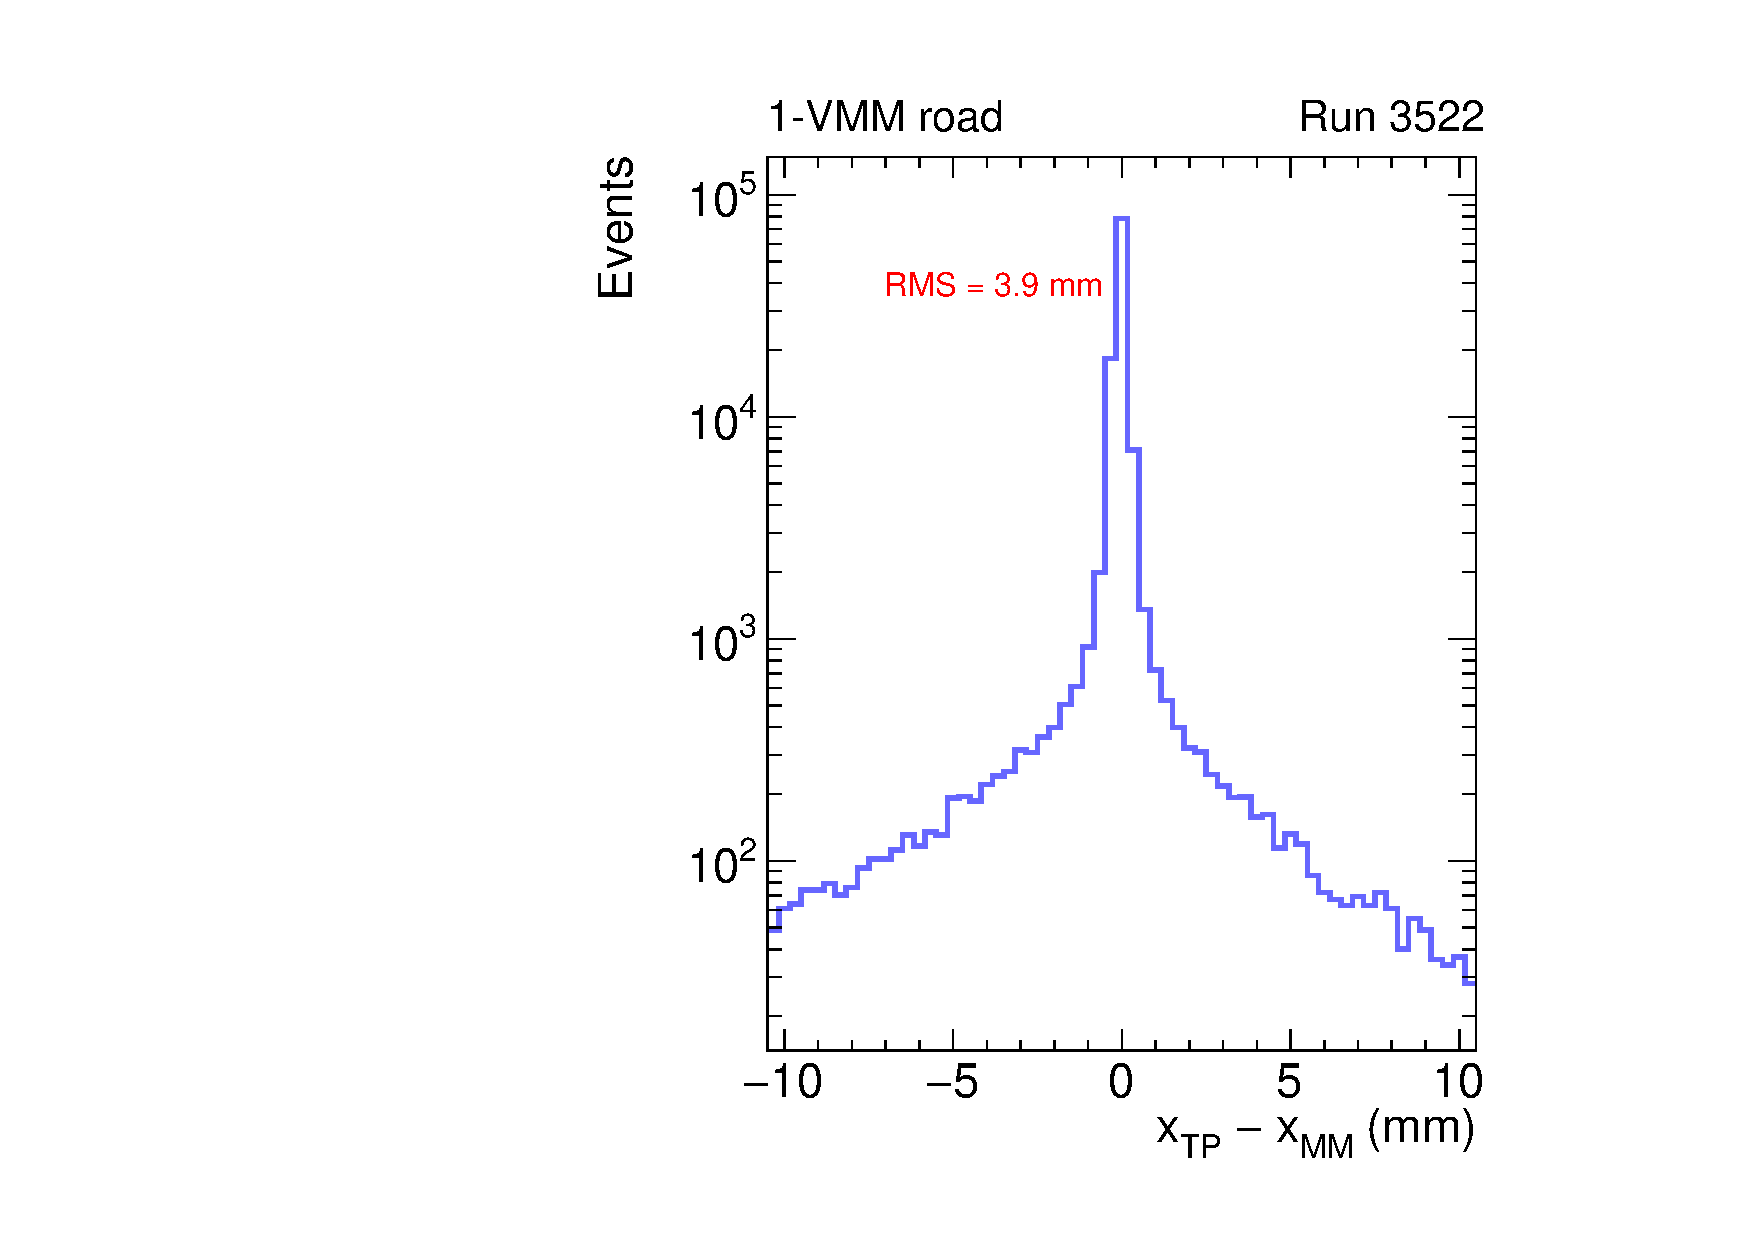
\includegraphics[width=0.4\textwidth]{figures/gbtanalysis3522/TP_xres_full.pdf}
    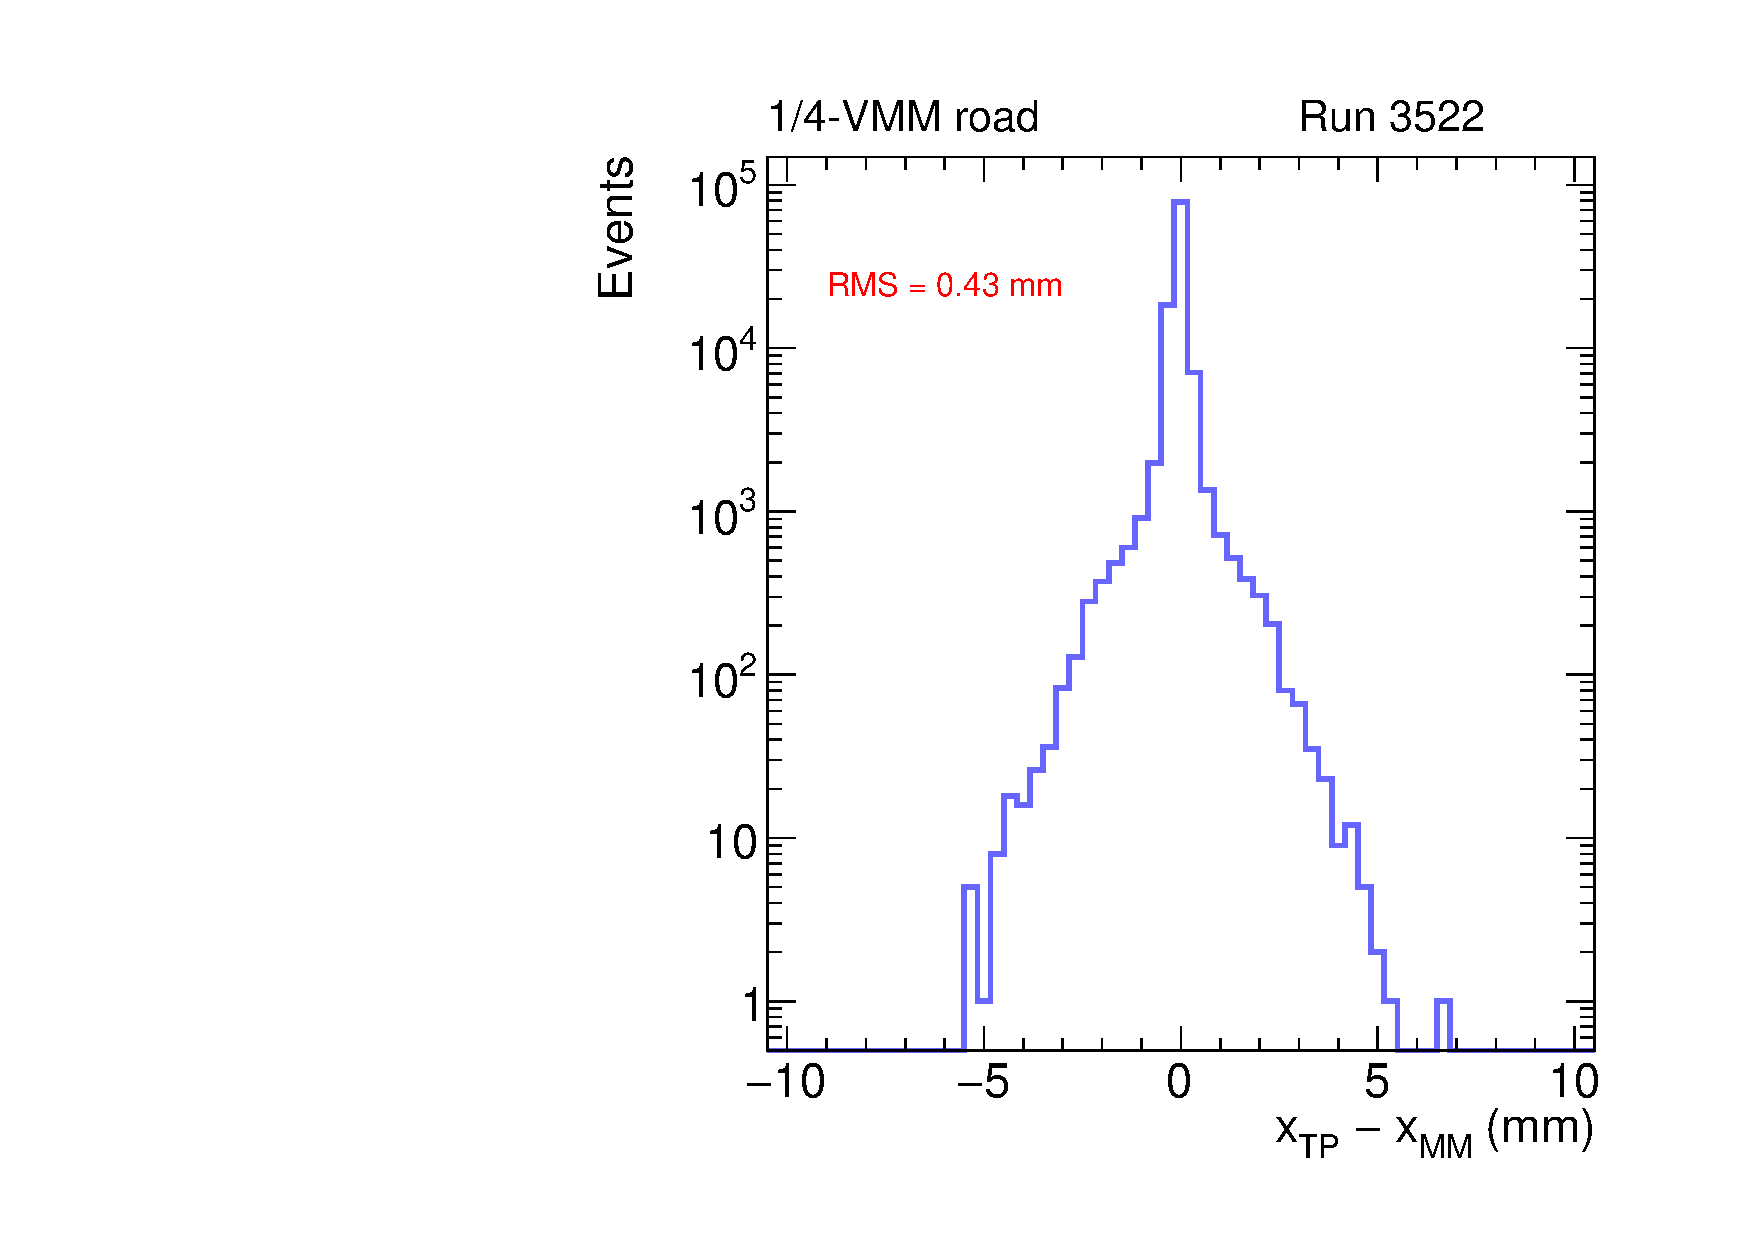
\includegraphics[width=0.4\textwidth]{figures/gbtanalysis3522/TP_xres.pdf}
  \end{center}
  \vspace{-10pt}
  \caption{The $x$ resolution of the MM TP relative to the full readout, using 1-VMM online roads (left) and 1/4-VMM offline roads (right). The tails of the resolution are greatly suppressed with smaller roads.}
  \label{fig:xres}
\end{figure}

\begin{figure}[!htpb]
  \begin{center}
    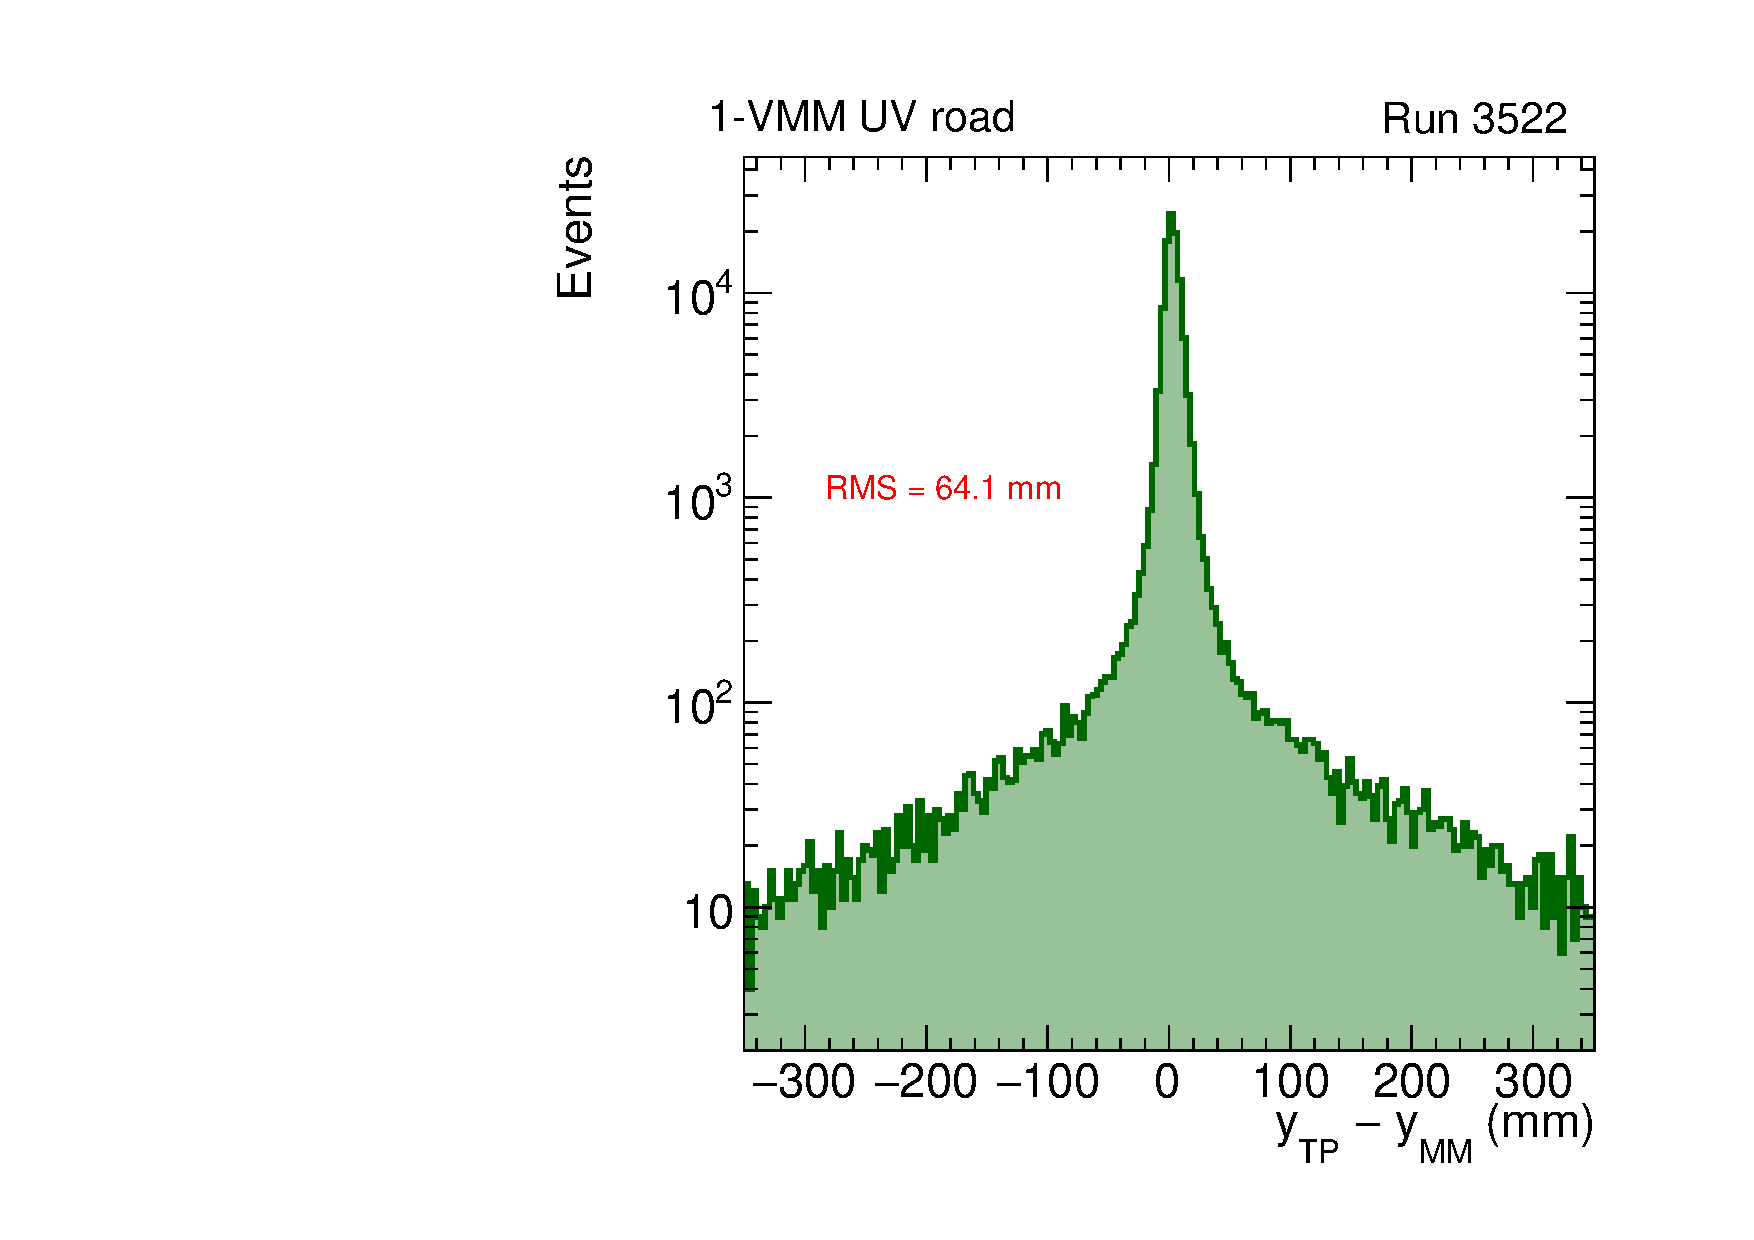
\includegraphics[width=0.4\textwidth]{figures/gbtanalysis3522/TP_yres_1road.pdf}
    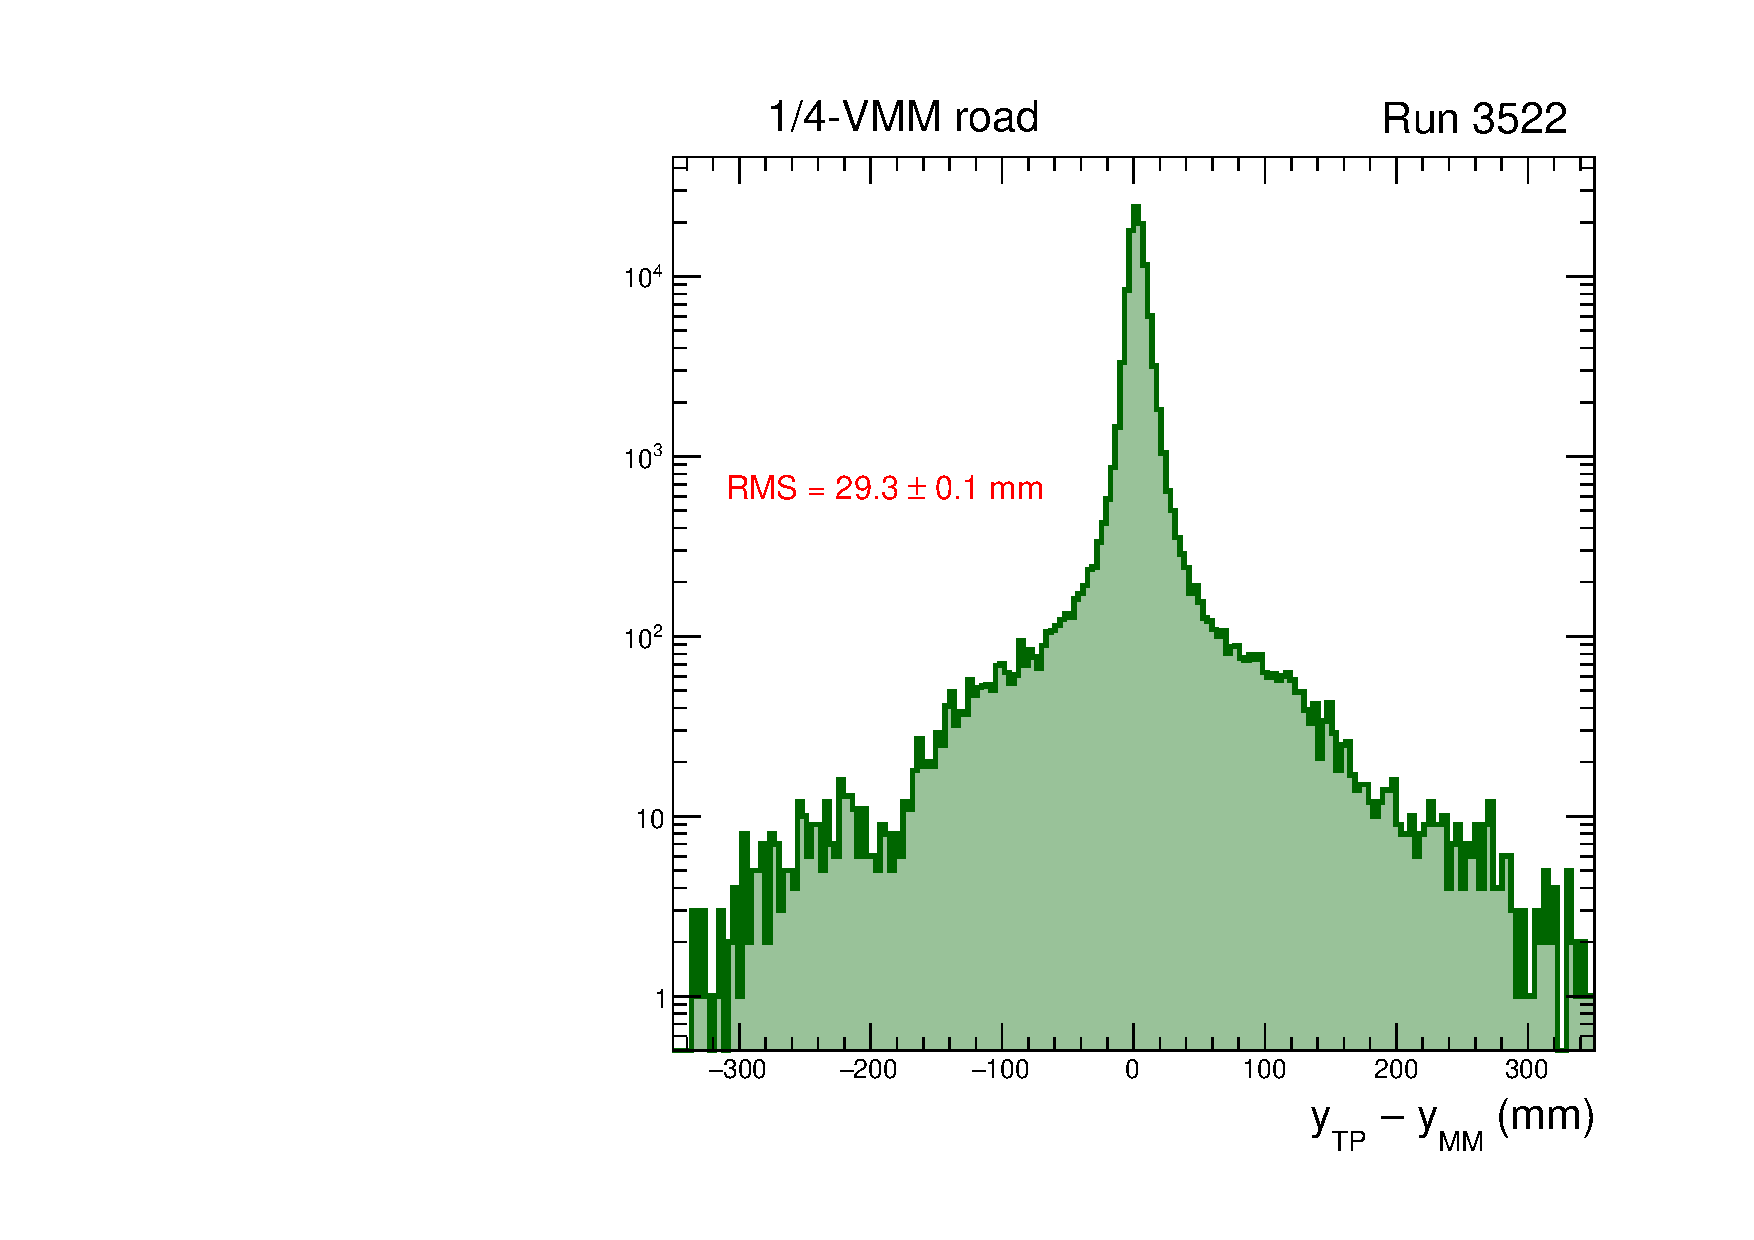
\includegraphics[width=0.4\textwidth]{figures/gbtanalysis3522/TP_yres_smallroad.pdf}
  \end{center}
  \vspace{-10pt}
  \caption{The $y$ resolution of the MM TP relative to the full readout, using 1-VMM online roads (left) and 1/4-VMM offline roads (right). The tails of the resolution are greatly suppressed with smaller roads.}
  \label{fig:yres}
\end{figure}

\begin{figure}[!htpb]
  \begin{center}
    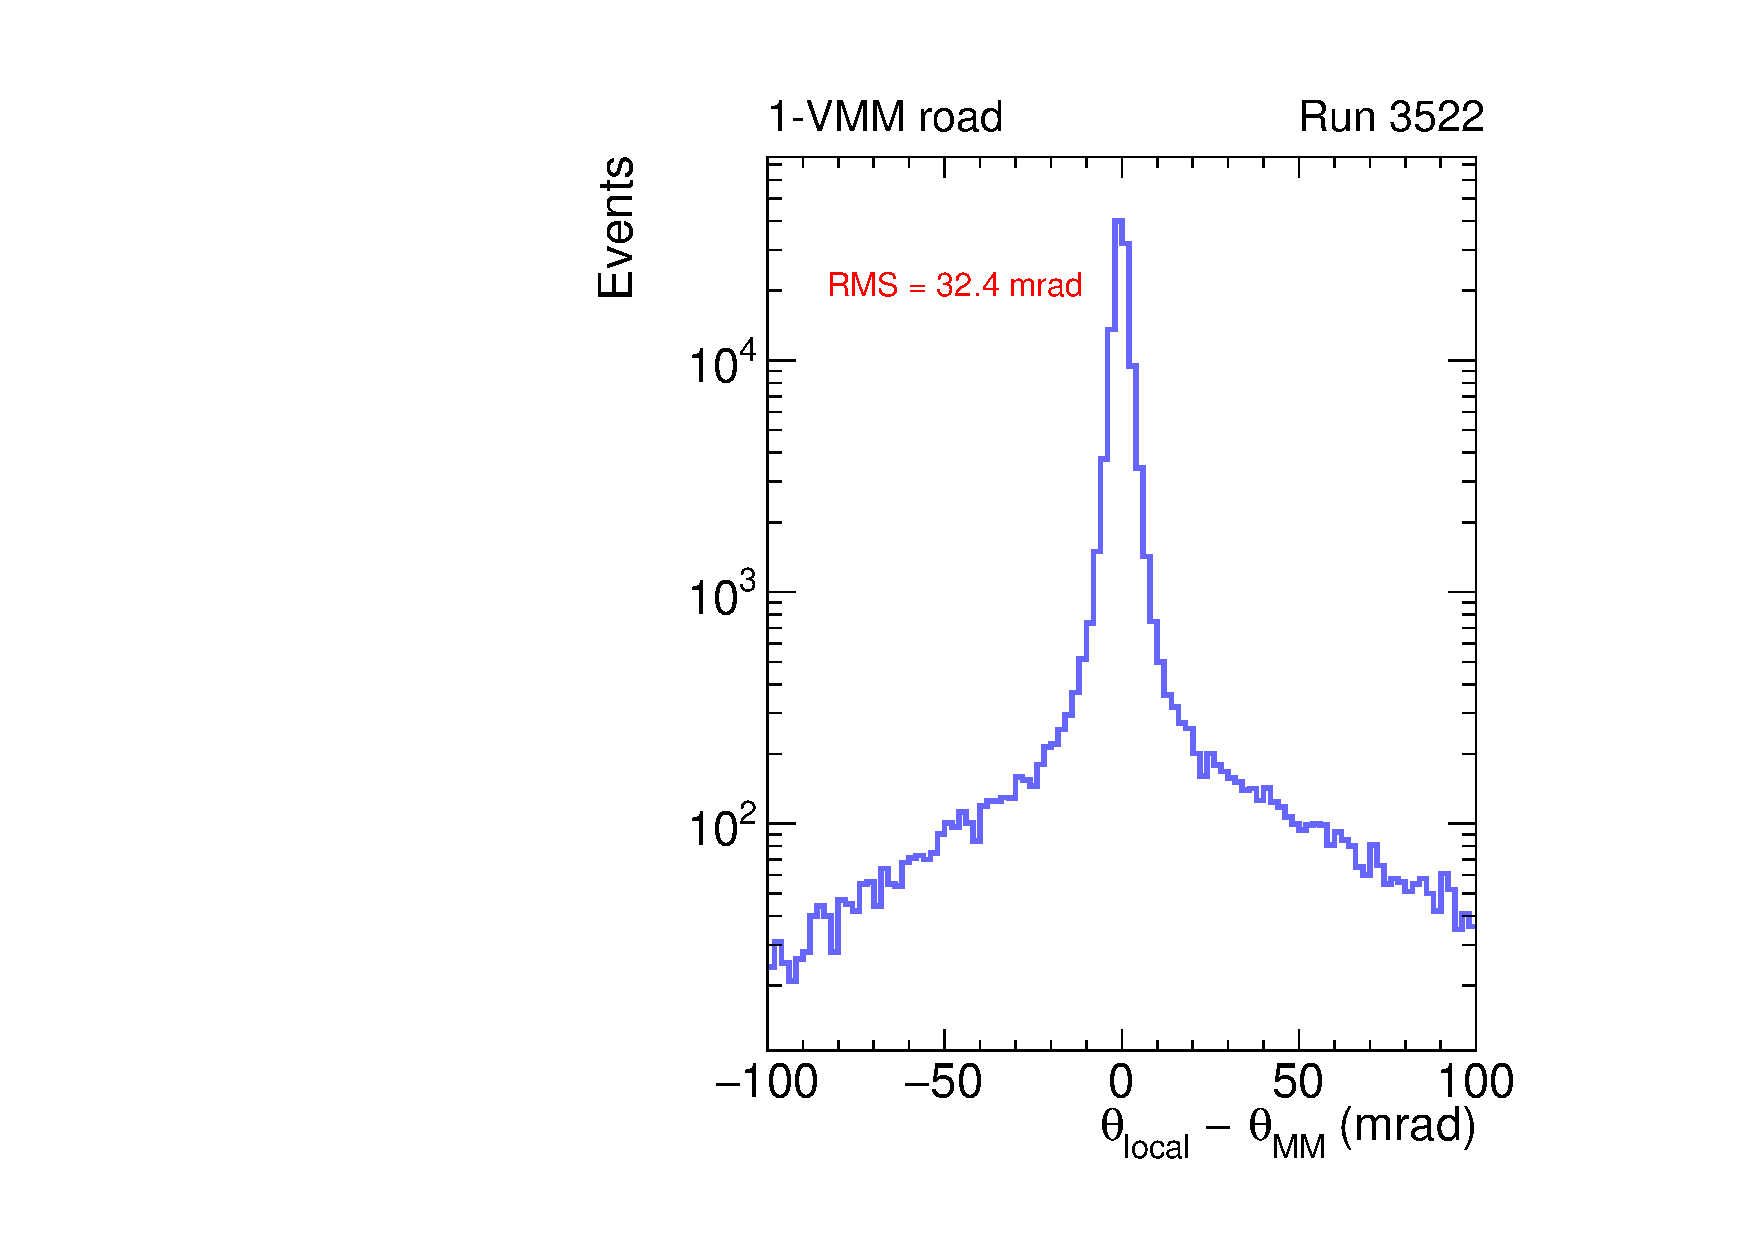
\includegraphics[width=0.4\textwidth]{figures/gbtanalysis3522/TP_angres_full.pdf}
    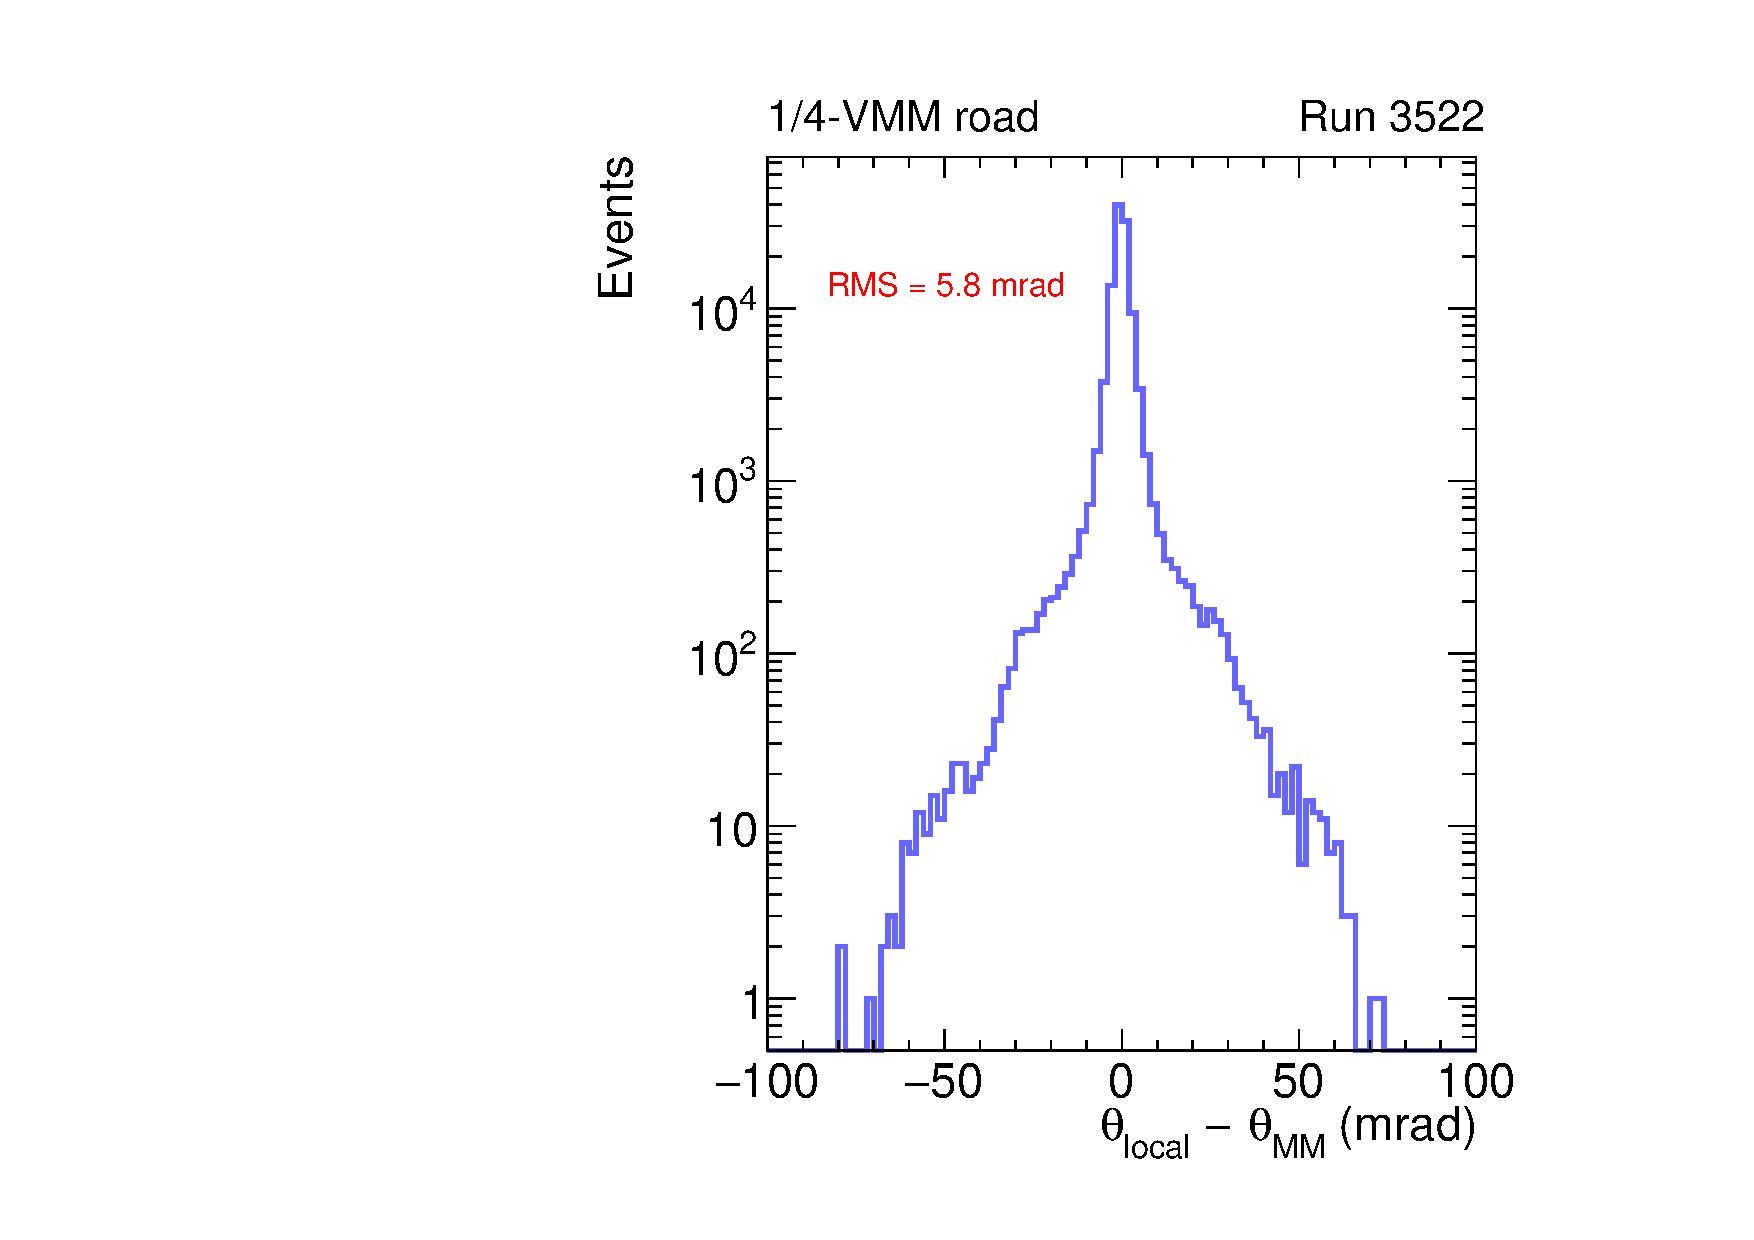
\includegraphics[width=0.4\textwidth]{figures/gbtanalysis3522/TP_angres.pdf}
  \end{center}
  \vspace{-10pt}
  \caption{The $\theta$ resolution of the MM TP relative to the full readout, using 1-VMM online roads (left) and 1/4-VMM offline roads (right). The tails of the resolution are greatly suppressed with smaller roads.}
  \label{fig:thetares}
\end{figure}


\subsubsection{Time resolution}

\begin{figure}[!htpb]
  \begin{center}
    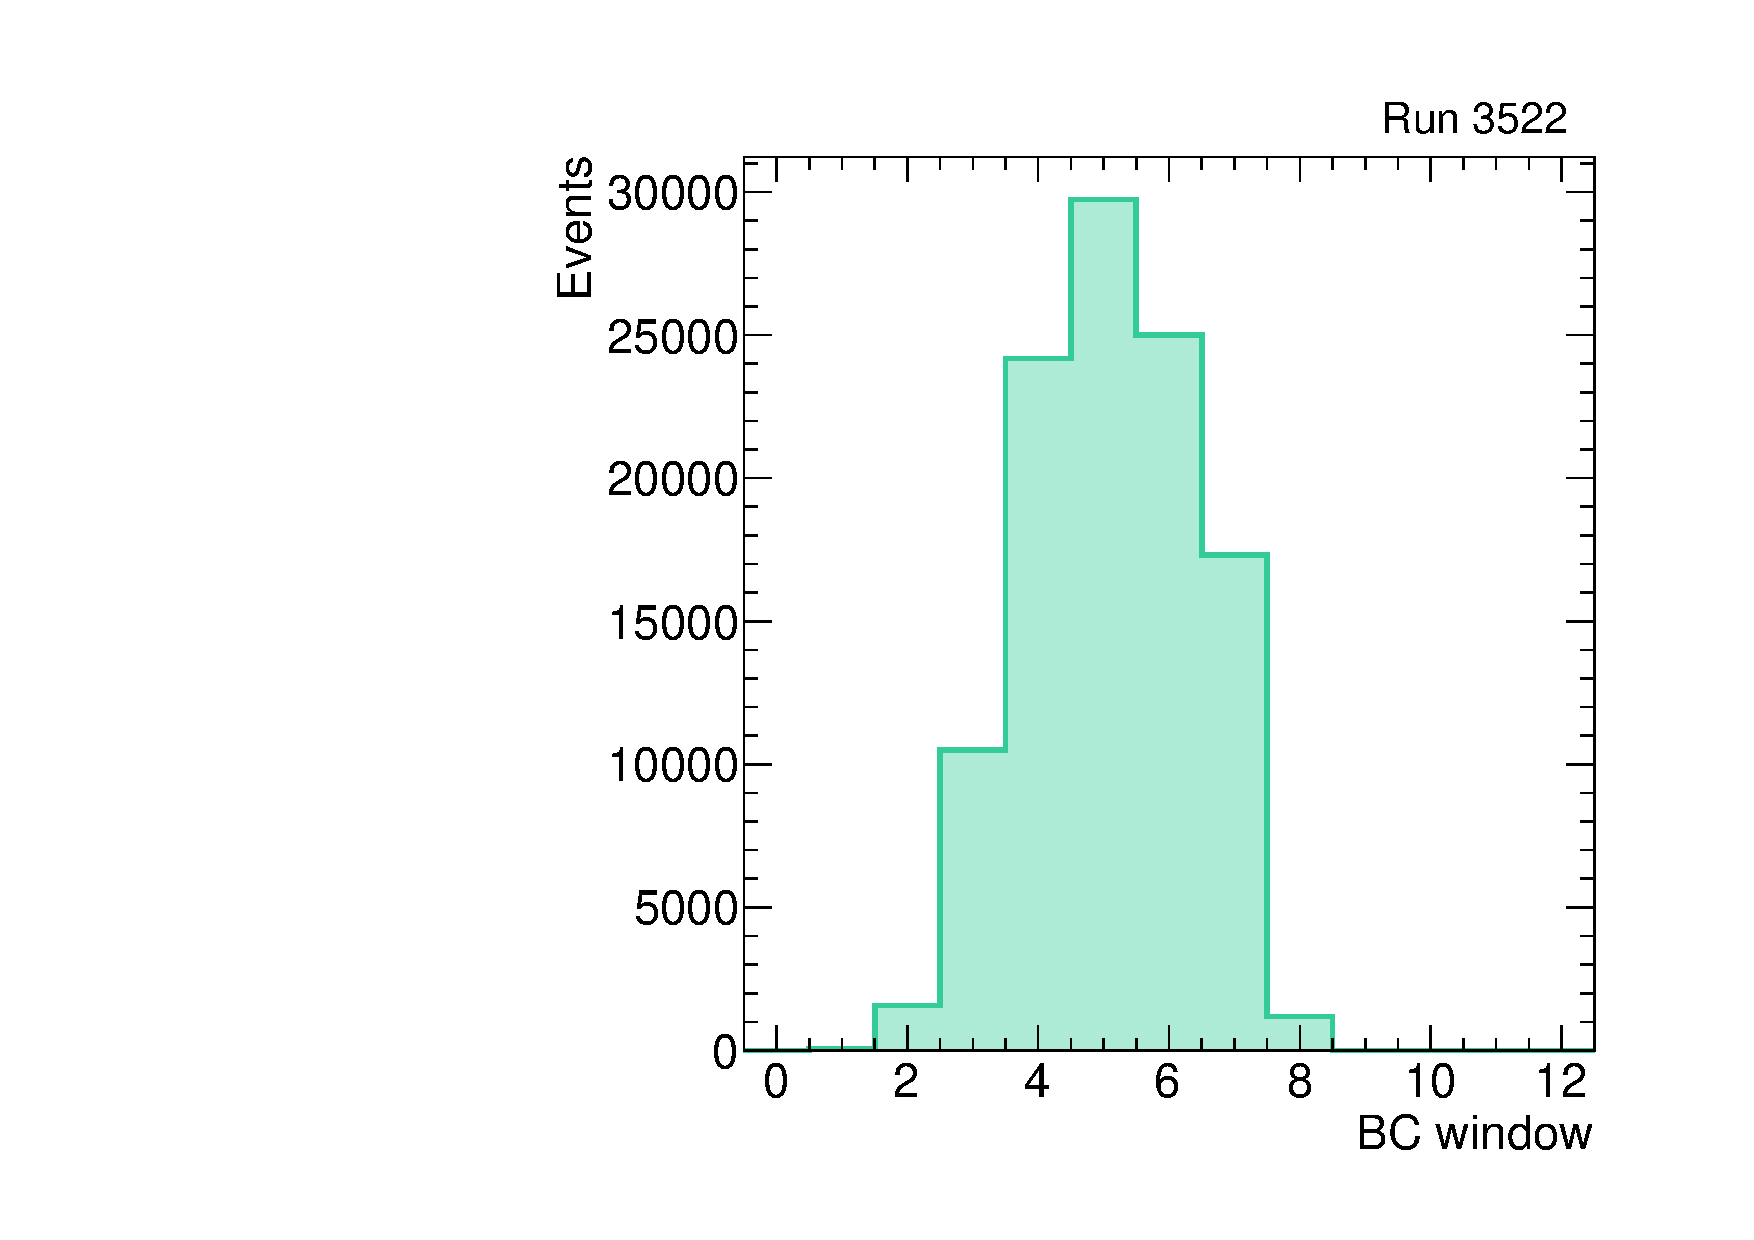
\includegraphics[width=0.4\textwidth]{figures/gbtanalysis3522/artwin_lin.pdf}
    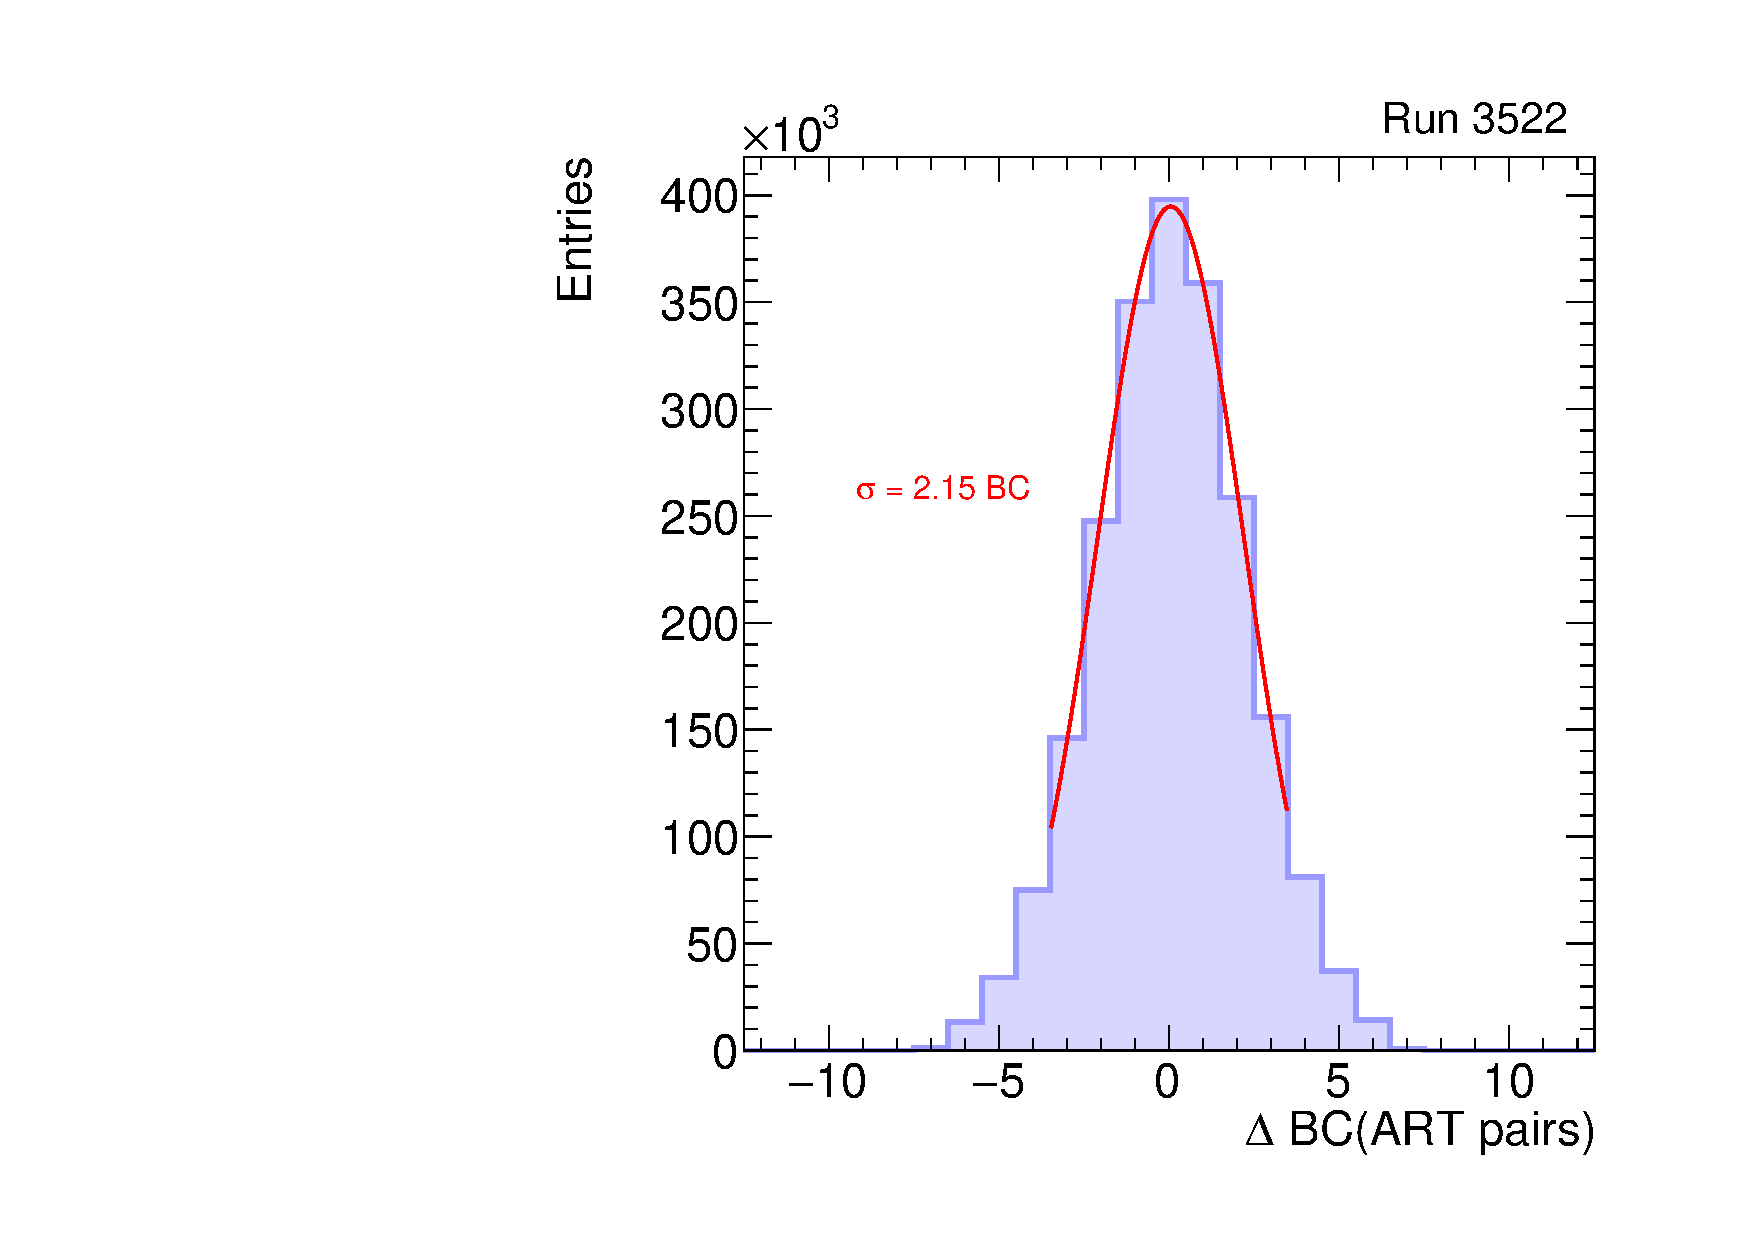
\includegraphics[width=0.4\textwidth]{figures/gbtanalysis3522/artrpairs_lin.pdf}
  \end{center}
  \vspace{-10pt}
  \caption{The time window required to record all hits in a trigger (left) and the $\Delta\text{BC}$ of all pairs of hits in a trigger (right). A gaussian fit is overlaid on the distribution of $\Delta\text{BC}$ and describes the data well.}
  \label{fig:time}
\end{figure}

\begin{figure}[!htpb]
  \begin{center}
    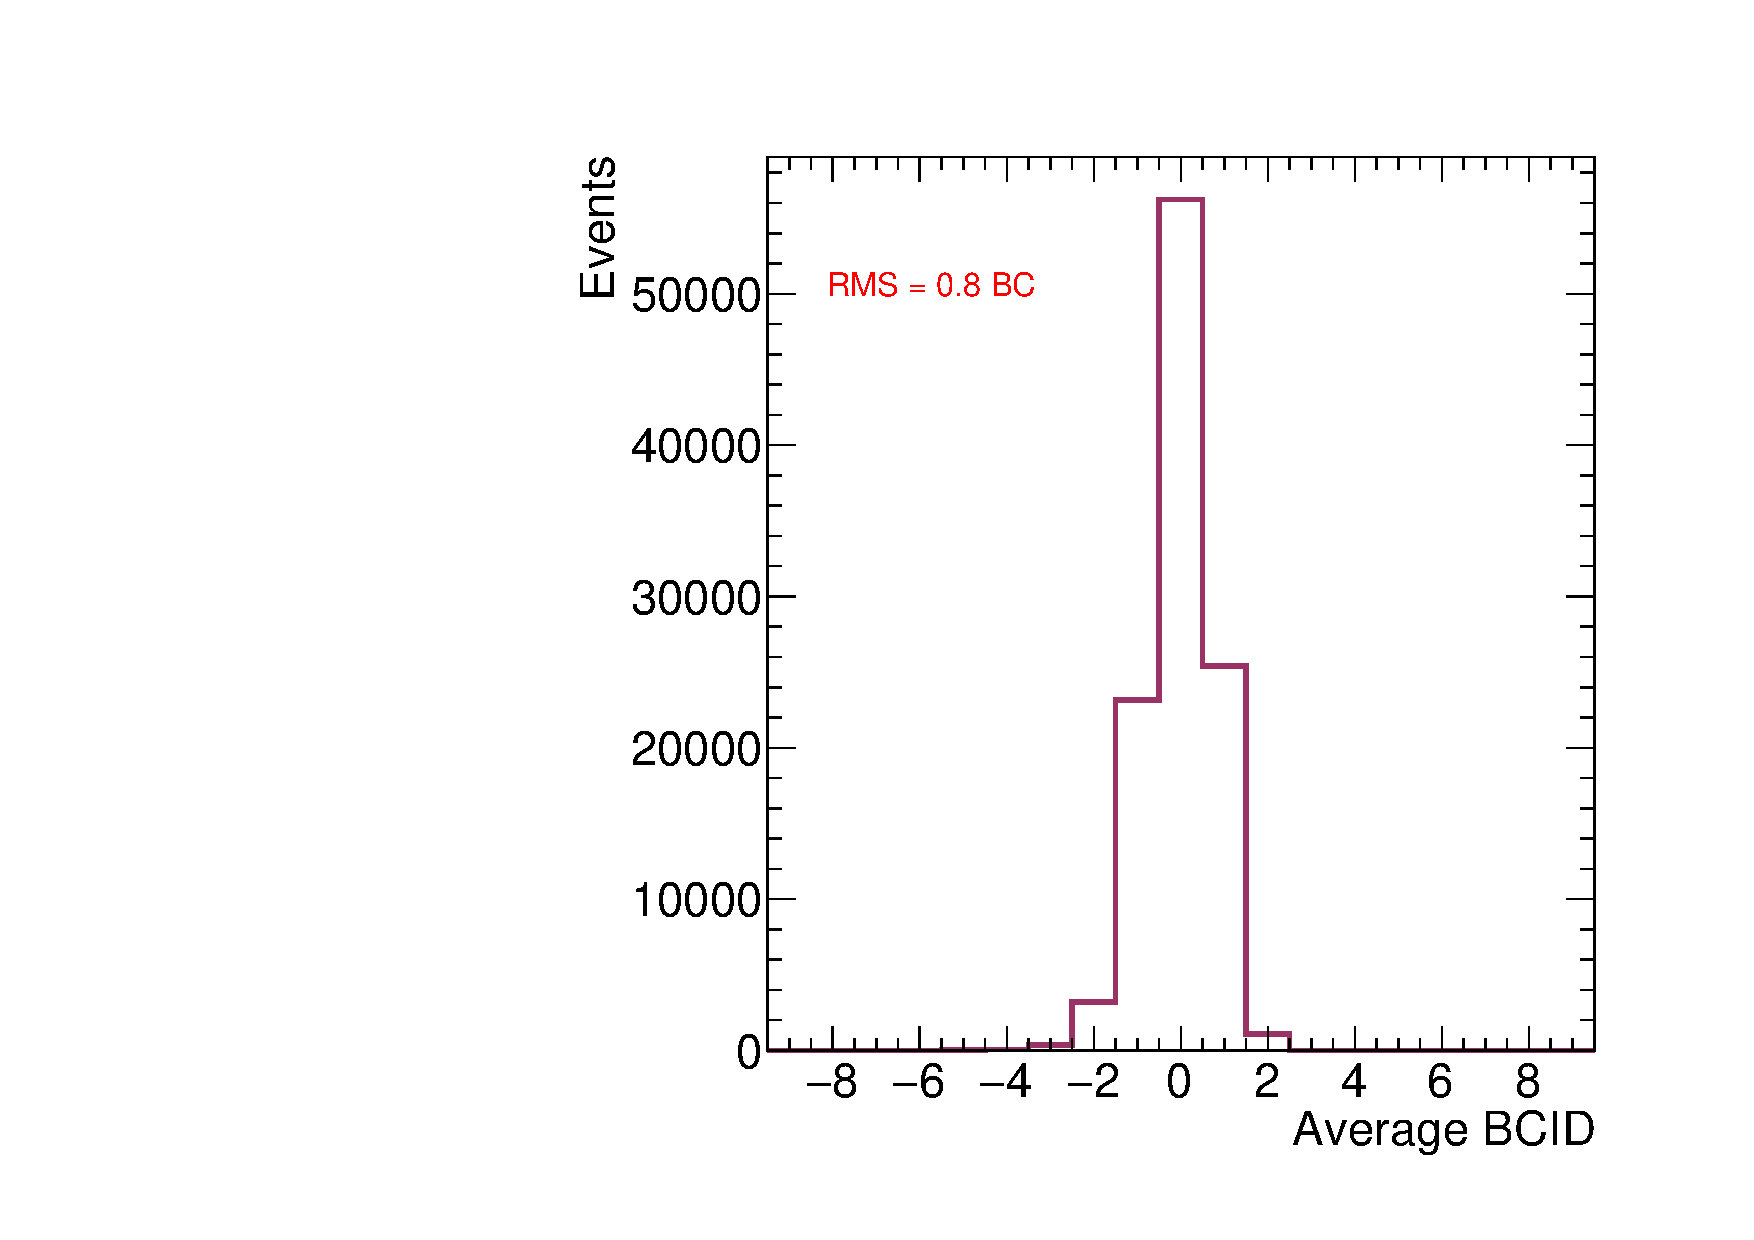
\includegraphics[width=0.4\textwidth]{figures/gbtanalysis3522/avg_BCID.pdf}
    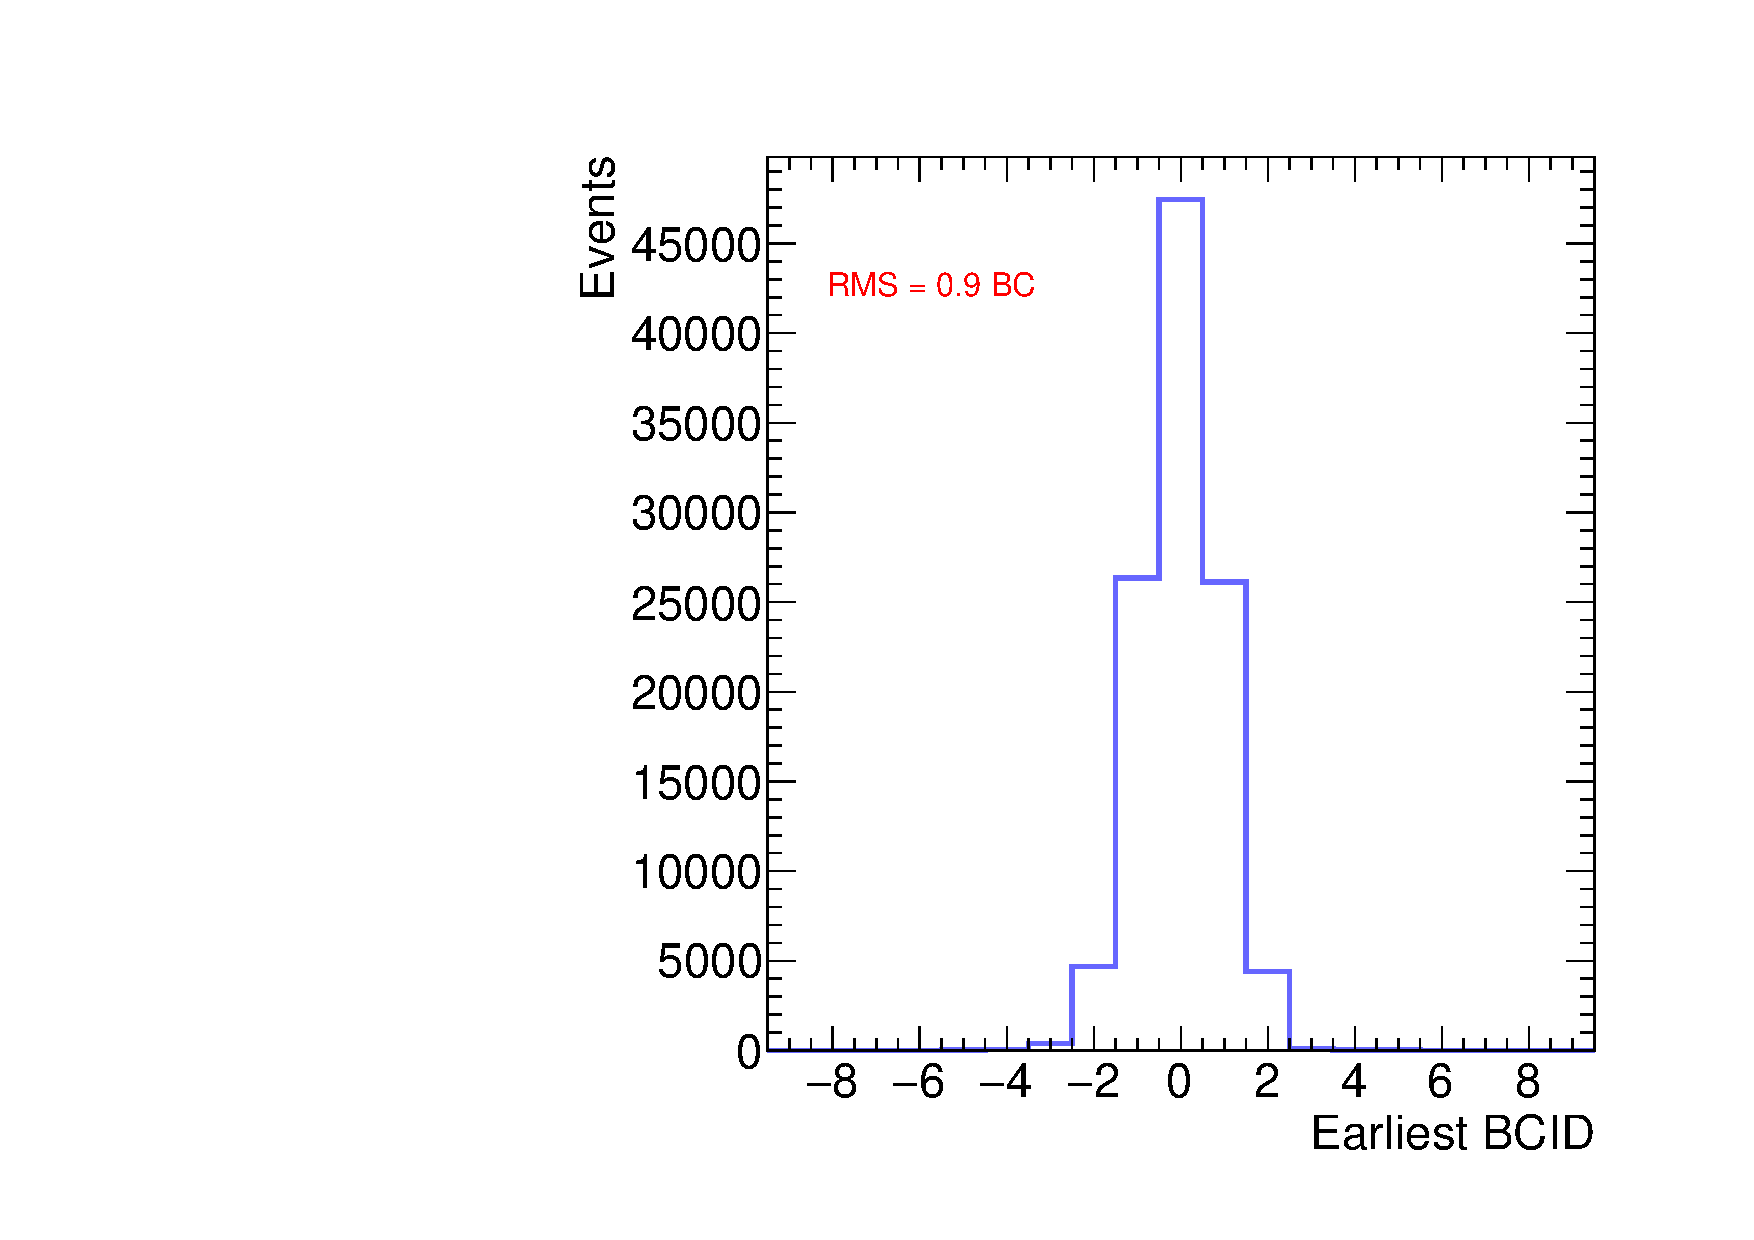
\includegraphics[width=0.4\textwidth]{figures/gbtanalysis3522/earliest_BCID.pdf}
  \end{center}
  \vspace{-10pt}
  \caption{The time resolution of the MM TP relative to the scintillator. The BCID of the trigger can be defined as the average BCID of the ART hits (left) or the earliest BCID (right). Choosing the average BCID has better resolution than choosing the earliest.}
  \label{fig:timeres}
\end{figure}

\subsection{Integration time}
\label{sec:perf-integ}


\section{Conclusion}
\label{sec:conclusions}

The performance of the Micromegas Address in Real Time (ART) and trigger processor is shown. The performance is measured with hundreds of thousands of cosmic muons in a low-background environment at the Harvard cosmic ray test stand. The test stand employs a full trigger electronics path with prototype hardware: MMFE8s equipped with VMM2, the FPGA-based ADDC V1, and a Micromegas trigger processor (MMTP) implemented on a VC707 FPGA evaluation board.

Given a track identified by the full front-end MMFE8 readout, the efficiency of the Micromegas trigger is $>\! 99\%$. The spatial, angular, and time resolution of the MMTP is measured with the front-end readout as reference, and the spatial and angular resolutions are found to be comparable to predictions made in the TDR. The time resolution is worse than predicted. The time resolution improves with shorter integration time; however, even with the shortest integration time considered, the time resolution is worse than anticipated.



\clearpage

\begin{thebibliography}{99}
\label{bibliography}
\setlength{\itemsep}{1.5pt plus 2.0pt minus 1.4pt}
\setlength{\parsep}{0pt}
\setlength{\parskip}{0pt}
\vspace{-6pt}

\bibitem{brian} B.~Clark et. al. An Algorithm for Micromegas Segment Reconstruction in the Level-1 Trigger of the New Small Wheel. \href{https://cds.cern.ch/record/1706160}{\color{blue}\underline{ATL-COM-UPGRADE-2014-012}}.
\bibitem{steve} S.~Chan et. al. Micromegas Trigger Processor Algorithm Performance in Nominal, Misaligned, and Misalignment Corrected Conditions. \href{https://cds.cern.ch/record/2113121}{\color{blue}\underline{ATL-COM-UPGRADE-2015-033}}.
\bibitem{noisy} P.~Giromini et. al. Performance of a Micromegas octuplet in the time of MMFE8 noise. \href{https://cds.cern.ch/record/2272355}{\color{blue}\underline{ATL-COM-MUON-2017-036}}.
\bibitem{noiseless} P.~Giromini et. al. Performance of a Micromegs octuplet after removing the major cause of noise. \href{https://cds.cern.ch/record/2277316}{\color{blue}\underline{ATL-COM-MUON-2017-040}}.
\bibitem{nswtdr} ATLAS New Small Wheel Technical Design Report. \href{http://cds.cern.ch/record/1552862}{\color{blue}\underline{ATLAS-TDR-020}}.
\bibitem{koki} Simulation of the ATLAS New Small Wheel (NSW) System. \href{http://cds.cern.ch/record/2265067}{\color{blue}\underline{ATL-MUON-SLIDE-2017-248}}.

\end{thebibliography}










\end{document} 

